\documentclass[UTF8,fontset=none,12pt]{ctexart}

\setCJKmainfont{Songti SC}
\setCJKsansfont{PingFang SC}
\setCJKmonofont{Songti SC}

\usepackage[a4paper,margin=2.35cm]{geometry}
\usepackage{amsmath,amssymb,amsthm,mathtools,bm}
\usepackage{graphicx}
\usepackage{float}
\usepackage{booktabs}
\usepackage{array}
\usepackage{enumitem}
\usepackage[hidelinks]{hyperref}

\title{数值线性代数\quad 第 40 讲：预处理}
\author{Lloyd N. Trefethen、David Bau III\\中文阅读版}
\date{}

\begin{document}
\maketitle

\noindent
\textbf{原书页码：}313--320；\quad
\textbf{目标 PDF 页码：}328--335（第 335 页为空白尾页）。

矩阵迭代的收敛取决于矩阵的性质：特征值、奇异值，有时还取决于其他信息。20 世纪
70、80 年代，迭代方法能够迅速发展的一个重要原因，是人们发现许多问题都可以先做
变换，使矩阵的这些性质得到大幅改善。这个过程称为\textbf{预处理}（preconditioning），
它是绝大多数成功应用迭代方法的关键。

\section*{$Ax=b$ 的预处理器}

抽象地说，为线性方程组预处理的想法很简单。设我们希望求解非奇异的
$m\times m$ 方程组

\begin{equation}
Ax=b.
\tag{40.1}
\end{equation}

对任意非奇异的 $m\times m$ 矩阵 $M$，方程组

\begin{equation}
M^{-1}Ax=M^{-1}b
\tag{40.2}
\end{equation}

与原方程组具有相同的解。但如果迭代求解式（40.2），收敛将取决于 $M^{-1}A$
的性质，而不是 $A$ 的性质。如果预处理器 $M$ 选择得好，式（40.2）可能比
式（40.1）快得多。

当然，要让这个想法有用，就必须能够高效地计算乘积 $M^{-1}A$ 所代表的操作。
和数值线性代数中的通常做法一样，这并不意味着显式构造逆矩阵 $M^{-1}$，而是
求解形如

\begin{equation}
My=c
\tag{40.3}
\end{equation}

的线性系统。

两个极端情形很容易想到。若 $M=A$，则式（40.3）与原问题（40.1）相同，应用
预处理器和直接求解原问题一样困难，什么也没有得到。若 $M=I$，则式（40.2）
与式（40.1）相同，应用预处理器虽然是小事，却没有产生任何效果。位于两者之间
的有效预处理器，应当具有足够结构，使式（40.3）可以快速求解；同时又要在某种
意义上足够接近 $A$，使式（40.2）的迭代比式（40.1）的迭代收敛更快。

那么，$M$ “足够接近 $A$”究竟是什么意思？这个问题其实贯穿了本书这一部分。
如果 $M^{-1}A$ 的特征值接近 1，并且
$\lVert M^{-1}A-I\rVert_2$ 很小，那么我们讨论过的任何一种迭代都可以期待快速
收敛（见习题 40.1）。不过，不满足这样强条件的预处理器也可能表现良好。例如，
$M^{-1}A$ 的特征值可以聚集在某个不等于 1 的数附近，同时允许少数远离主体的离群
特征值。又例如，如果采用 CGN，只要 $M^{-1}A$ 的奇异值聚集即可，不必要求特征值
聚集。

和往常一样，收敛速率的精细分析归结为复平面上的多项式逼近问题。与基本迭代相比，
预处理器分析中唯一改变的是：现在关注的不是 $A$ 的性质，而是 $M^{-1}A$ 的性质。
对于除 CGN 以外的大多数迭代，一个简单经验法则通常就够用了：

\[
\boxed{\text{若 }M^{-1}A\text{ 不要过分偏离正规矩阵，且其特征值聚集，则 }M\text{ 是好的预处理器。}}
\]

\section*{左预处理、右预处理与 Hermitian 预处理}

上面描述的更准确名称是\textbf{左预处理}。另一种做法是把
$Ax=b$ 变换为

\[
AM^{-1}y=b,\qquad x=M^{-1}y,
\]

此时 $M$ 称为\textbf{右预处理器}。实际计算中左、右预处理器都会使用，有时还会
同时使用两者。为了简化讨论，本讲只考虑左预处理。

如果 $A$ 是 Hermitian 正定矩阵，预处理时通常希望保留这个性质。设 $M$ 也是
Hermitian 正定矩阵，并写成

\[
M=CC^*
\]

的形式。则式（40.1）等价于

\begin{equation}
\bigl[C^{-1}AC^{-*}\bigr]C^*x=C^{-1}b,
\qquad C^{-*}=(C^*)^{-1}.
\tag{40.4}
\end{equation}

方括号中的矩阵是 Hermitian 正定的，因此这个方程可以用 CG 或相关迭代求解。
同时注意到，$C^{-1}AC^{-*}$ 与

\[
C^{-*}C^{-1}A=M^{-1}A
\]

相似，所以为了研究收敛，只需考察非 Hermitian 矩阵 $M^{-1}A$ 的特征值。

\section*{例}

图 40.1 给出了一个对称正定矩阵上预处理 CG 迭代的例子。矩阵 $A$ 取自习题 36.3
的构造：它是一个 $1000\times1000$ 的对称矩阵，除下列元素外全部为零：

\[
a_{ij}=
\begin{cases}
0.5+\sqrt{i}, & i=j,\\
1, & |i-j|=1,\\
1, & |i-j|=100.
\end{cases}
\]

右端项取为 $b=(1,1,\ldots,1)^T$。如图所示，直接对这个矩阵运行 CG 收敛较慢；
迭代 40 步后，残量大约只减少了 5 位数字。由于矩阵非常稀疏，这已经优于直接
方法，但我们希望做得更好。

事实证明，一个简单的对角预处理器就能带来显著改进。取

\[
M=\operatorname{diag}(A),
\]

即对角线上元素为 $m_{ii}=0.5+\sqrt{i}$ 的对角矩阵。为了保持对称性，令
$C=M^{1/2}$，并采用式（40.4）中的预处理迭代。图中显示，此时只需 30 步左右
就能达到约 15 位数字的精度。

\begin{figure}[H]
\centering
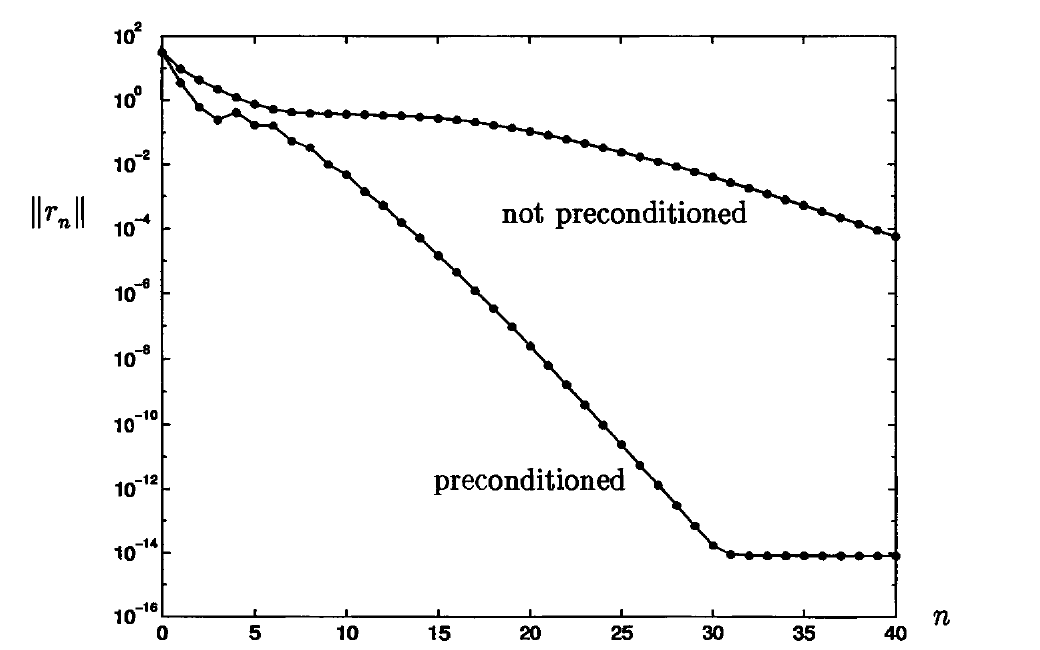
\includegraphics[width=0.88\textwidth]{../assets/figure-40-1-preconditioned-cg.png}
\parbox{0.94\textwidth}{\small 图 40.1. 文中所述 $1000\times1000$ 稀疏矩阵 $A$ 上
CG 与预处理 CG 的收敛曲线。矩阵是习题 36.3 的矩阵加上 $0.5I$；预处理后约 30 步
达到机器精度，而未预处理曲线在 40 步时仍明显较慢。}
\end{figure}

\section*{$Ax=b$ 的预处理器概览}

实际使用的预处理器有时和上面的对角预处理器一样简单，但往往复杂得多。本节不
详细研究一两个例子，而是反过来从较高层次概览这些年来已经证明有用的大量预处理
思想；具体细节可参见本书注释中列出的参考文献。

\paragraph{对角缩放或 Jacobi 预处理。}
也许最重要的预处理器就是刚才例子中的
$M=\operatorname{diag}(A)$，前提是这个矩阵非奇异。对某些问题，仅这一变换就足以
把缓慢迭代变成快速迭代。更一般地，也可以取

\[
M=\operatorname{diag}(c),
\qquad c\in\mathbb C^m
\]

其中 $c$ 是适当选择的向量。要确定一个使 $\kappa(M^{-1}A)$ 恰好最小的 $c$，
这是一个困难的数学问题；幸运的是，实践中不需要达到精确最小值，而且经验法则
也说明，预处理不只是最小化条件数。

\paragraph{不完全 Cholesky 或 LU 分解。}
另一个明星级预处理器正是不完全分解，它在 20 世纪 70 年代使预处理思想声名大振。
设 $A$ 稀疏，每行只有少量非零元。高斯消去或 Cholesky 分解的困难在于，它们会
破坏零元素：例如若 $A=R^*R$，因子 $R$ 通常就不再稀疏。

但是，可以按照 Cholesky 类似的公式计算一个矩阵 $\widetilde R$，只允许它在 $A$
已有非零元的位置出现非零元，并定义

\[
M=\widetilde R^*\widetilde R.
\]

这种不完全 Cholesky 预处理器对某些问题非常有效；“不完全 Cholesky 共轭梯度”
常缩写为 ICCG。类似地，非对称问题可以使用 ILU（不完全 LU）预处理器。围绕
不完全分解的思想，人们还提出并发展了许多变体。

这两个例子都没有利用底层问题 $Ax=b$ 的来源。不过，设计预处理器最有价值的一般
建议是：研究问题本身并利用它的结构。可以问：如果问题以某种方式变简单，是否就
能快速求解？如果可以，这个更简单的问题版本可能就是有效的预处理器。下面的大多
数例子都属于这一类。

\paragraph{粗网格近似。}
在细网格上离散偏微分方程或积分方程，可能会得到一个巨大的方程组；而在较粗网格
上做相同的离散，可能只产生一个容易求解的小系统。如果能找到一种方法（例如插值）
在粗网格与细网格之间来回传递解，就可以得到如下示意形式的强大预处理器：

\begin{equation}
M=(\text{传递到细网格})\circ A_{\text{coarse}}\circ
(\text{传递到粗网格}).
\tag{40.5}
\end{equation}

这类预处理器通常很擅长处理原问题的低频成分，把高频成分留给 Krylov 子空间迭代。
如果继续迭代这一技术，构造越来越粗的网格，就得到多重网格迭代的思想。

\paragraph{局部近似。}
粗网格近似考虑问题的大尺度结构，同时忽略一部分细节。与之相反的一种思想适用于
这样的 $Ax=b$：$A$ 表示相互作用，而元素之间既有近距离耦合，也有远距离耦合。
这些元素可以是粒子等物理对象，也可以是边界元离散中使用的面板等数值对象。
这时可以考虑构造一个与 $A$ 类似、但删除长程相互作用的算子 $M$，即 $A$ 的
短程近似。最简单的情形是，$M$ 只由 $A$ 主对角线附近的几条对角线组成，这就
推广了对角预处理器的思想。

\paragraph{块预处理器与区域分解。}
在数值线性代数中，几乎所有用矩阵标量元素表达的算法，都有块矩阵版本。例如，
对角或 Jacobi 预处理器可以推广为块对角或块 Jacobi 形式。这也是一种局部近似：
只考虑某些组件内部的局部影响，而忽略它们与其他组件之间的连接。

近些年，这类思想在区域分解领域得到了广泛推广：把针对某些子区域的求解器以灵活
方式组合起来，形成全局问题的预处理器。这些方法兼具数学力量和天然的并行性。

\paragraph{低阶离散。}
微分方程或积分方程常常用四阶有限差分公式或谱方法等高阶方法离散。这样可以提高
精度，却会使离散模板更大、矩阵更不稀疏。同一问题的低阶近似具有更稀疏的矩阵，
可能成为有效的预处理器。因此，谱离散中常能见到有限差分和有限元预处理器。

\paragraph{常系数或对称近似。}
对于常系数偏微分方程，有快速 Poisson 求解器等特殊技术。若问题具有变系数，
则可以用快速求解器实现一个常系数近似，并把它用作预处理器。类似地，如果某个
微分方程不是自伴的，但在某种意义上接近一个更容易求解的自伴方程，后者有时也能
充当预处理器。

\paragraph{多项算子分裂。}
许多应用包含多种物理效应的组合，例如扩散和对流共同构成流体力学中的 Navier--Stokes
方程。在线性代数层面，这可能表现为

\[
A=A_1+A_2
\]

的矩阵问题 $Ax=b$（当然也可能有两个以上的项），并且常常嵌入非线性迭代中。
如果 $A_1$ 或 $A_2$ 容易求逆，它就可能成为好的预处理器。

\paragraph{维度分裂或 ADI。}
另一种分裂利用这样的事实：二维或三维 Laplace 算子可以分解为各个坐标方向上
分别作用的类似算子。这一思想可以作为预处理器的基础；它的一种形式称为 ADI，
即交替方向隐式（alternating direction implicit）方法。

\paragraph{经典迭代的一步。}
本书没有讨论 Jacobi、Gauss--Seidel、SOR 或 SSOR 等“经典迭代”，但这些迭代的
一步或多步（尤其是 Jacobi 和 SSOR）常常能很好地充当预处理器。这也是多重网格
方法背后的关键思想之一。

\paragraph{周期或卷积近似。}
在数学科学中，边界条件是分析和计算困难的来源。如果没有边界条件、问题定义在
周期区域上，情况会简单得多；这个想法有时可以构成一个好的预处理器。

在线性代数最简单的情形中，考虑 Toeplitz 矩阵 $A$，即

\[
a_{ij}=a_{i-j},
\]

用相关的循环矩阵 $M$ 进行预处理，其中

\[
m_{ij}=m_{(i-j)\bmod m}.
\]

循环矩阵可以通过快速 Fourier 变换在 $O(m\log m)$ 次运算中求逆。这是一个特别
值得研究的例子：$M^{-1}A$ 在范数意义上可能离单位矩阵很远，但其特征值却高度聚集。

\paragraph{不稳定的直接方法。}
某些数值方法（如不选主元的高斯消去）由于不稳定会给出不准确的答案。然而，如果
这个不稳定方法很快，为什么不把它用作预处理器？这就是数值计算中的“飞线控制”
（fly by wire）思想：先粗心但快速地求解问题，再把这个解嵌入一个稳健的控制系统
中。这是一个很有力的想法。

\paragraph{多项式预处理器。}
最后介绍一种与其他方法不同的技术：预处理器本质上近似的不是 $A$，而是 $A^{-1}$。
多项式预处理器是一个矩阵多项式

\[
M^{-1}=p(A),
\]

它使 $p(A)A$ 比 $A$ 本身更适合迭代。例如，$p(A)$ 可以取自 Neumann 级数
的前几项：

\[
A^{-1}=I+(I-A)+(I-A)^2+\cdots,
\]

也可以来自其他表达式，通常由复平面上的逼近理论启发。它很容易实现，因为可以
使用与 Krylov 子空间迭代相同的“黑箱”；预处理器的系数有时还可以自适应确定。

\section*{特征值问题的预处理器}

虽然这一思想发展得较晚，知名度也还不如线性方程组中的预处理，但预处理器同样
可以有效地处理特征值问题。这里最著名的一些技术包括：与前面线性方程组中的多项
式预处理相对应的多项式加速；使用 $A$ 的有理函数而非多项式的 shift-and-invert
Arnoldi 或相关的有理 Krylov 迭代；以及建立在某种对角预处理器基础上的 Davidson
方法和 Jacobi--Davidson 方法。

例如，shift-and-invert 和有理 Krylov 方法利用如下事实：若 $r(z)$ 是有理函数，
且 $\{\lambda_j\}$ 是 $A$ 的特征值，那么 $r(A)$ 的特征值就是

\[
\{r(\lambda_j)\}.
\]

如果能够以合理速度计算 $r(A)$，并且其特征值比 $A$ 的特征值更适合迭代，那么这
就可能成为快速计算特征值的一条路线。

\section*{结语}

本书以预处理器为主题收尾，我们也就此触及未来科学计算的哲学中心。计算机科学家
的传统观点是：一个计算问题是有限的；经过一段或长或短的计算，最终可以精确得到
解。然而，多年来，这种观点适用的问题越来越少。大规模计算问题的最佳方法通常是
近似方法：在较短时间内得到令人满意的准确解，而不是用更长、甚至无限长的时间
得到精确解。

数值分析确实首先是分析的一个分支，而不是代数的分支，即使所求解的问题来自线性
代数。附录还会对这一现象作进一步思考。

在下一个世纪的科学计算中，没有什么会比这样的技艺更核心：把看似不可处理的问题
变换为另一个可以快速近似求解的问题。对于 Krylov 子空间矩阵迭代，这种技艺就是
预处理。对于范围广泛的连续与离散计算问题，我们只能猜测这一思想最终会把我们
带向何方。

\section*{习题}

\paragraph{40.1.}
设 $A=M-N$，其中 $M$ 非奇异。假设

\[
\lVert I-M^{-1}N\rVert_2\leq\frac12,
\]

并像式（40.2）那样使用 $M$ 作为预处理器。

\begin{enumerate}[label=(\alph*)]
\item 证明对这个预处理问题应用 GMRES 后，20 步迭代的残量范数保证至少缩小六个数量级。
\item 为得到同样的保证，需要进行多少步 CGN？
\end{enumerate}

\paragraph{40.2.}
证明：如果矩阵 $A$ 和预处理器 $M$ 都是 Hermitian 正定的，那么无论把 $M$ 用作
左预处理器还是右预处理器，都能得到相同的 CG 收敛速率。解释为什么对于非 Hermitian
矩阵以及 GMRES、CGN 或 BCG 这样的迭代，这个结论不再成立。

\end{document}
